%%%%%%%%%%%%%%%%%%%%%%%%%%%%%%%%%%%%%%%%%
% Arsclassica Article
% LaTeX Template
% Version 1.1 (10/6/14)
%
% This template has been downloaded from:
% http://www.LaTeXTemplates.com
%
% Original author:
% Lorenzo Pantieri (http://www.lorenzopantieri.net) with extensive modifications by:
% Vel (vel@latextemplates.com)
%
% License:
% CC BY-NC-SA 3.0 (http://creativecommons.org/licenses/by-nc-sa/3.0/)
%
%%%%%%%%%%%%%%%%%%%%%%%%%%%%%%%%%%%%%%%%%

%----------------------------------------------------------------------------------------
%	PACKAGES AND OTHER DOCUMENT CONFIGURATIONS
%----------------------------------------------------------------------------------------

\documentclass[
12pt, % Main document font size
a4paper, % Paper type, use 'letterpaper' for US Letter paper
oneside, % One page layout (no page indentation)
%twoside, % Two page layout (page indentation for binding and different headers)
headinclude,footinclude, % Extra spacing for the header and footer
BCOR5mm, % Binding correction
]{scrartcl}

%%%%%%%%%%%%%%%%%%%%%%%%%%%%%%%%%%%%%%%%%
% Arsclassica Article
% Structure Specification File
%
% This file has been downloaded from:
% http://www.LaTeXTemplates.com
%
% Original author:
% Lorenzo Pantieri (http://www.lorenzopantieri.net) with extensive modifications by:
% Vel (vel@latextemplates.com)
%
% License:
% CC BY-NC-SA 3.0 (http://creativecommons.org/licenses/by-nc-sa/3.0/)
%
%%%%%%%%%%%%%%%%%%%%%%%%%%%%%%%%%%%%%%%%%

%----------------------------------------------------------------------------------------
%	REQUIRED PACKAGES
%----------------------------------------------------------------------------------------

\usepackage[
nochapters, % Turn off chapters since this is an article        
beramono, % Use the Bera Mono font for monospaced text (\texttt)
eulermath,% Use the Euler font for mathematics
pdfspacing, % Makes use of pdftex’ letter spacing capabilities via the microtype package
dottedtoc % Dotted lines leading to the page numbers in the table of contents
]{classicthesis} % The layout is based on the Classic Thesis style

\usepackage{arsclassica} % Modifies the Classic Thesis package

\usepackage[T1]{fontenc} % Use 8-bit encoding that has 256 glyphs

\usepackage[utf8]{inputenc} % Required for including letters with accents

\usepackage{graphicx} % Required for including images
\graphicspath{{Figures/}} % Set the default folder for images

\usepackage{enumitem} % Required for manipulating the whitespace between and within lists

\usepackage{lipsum} % Used for inserting dummy 'Lorem ipsum' text into the template

\usepackage{subfig} % Required for creating figures with multiple parts (subfigures)

\usepackage{amsmath,amssymb,amsthm} % For including math equations, theorems, symbols, etc

\usepackage{varioref} % More descriptive referencing

\usepackage{tabularx} % http://tex.stackexchange.com/questions/15282/tabular-title-above-and-caption-below
\usepackage{ragged2e}
\usepackage{booktabs}
\usepackage{caption}

\usepackage{url} % http://stackoverflow.com/questions/2640111/url-latex-linebreak-problem

%----------------------------------------------------------------------------------------
%	THEOREM STYLES
%---------------------------------------------------------------------------------------

\theoremstyle{definition} % Define theorem styles here based on the definition style (used for definitions and examples)
\newtheorem{definition}{Definition}

\theoremstyle{plain} % Define theorem styles here based on the plain style (used for theorems, lemmas, propositions)
\newtheorem{theorem}{Theorem}

\theoremstyle{remark} % Define theorem styles here based on the remark style (used for remarks and notes)

%----------------------------------------------------------------------------------------
%	HYPERLINKS
%---------------------------------------------------------------------------------------

\hypersetup{
%draft, % Uncomment to remove all links (useful for printing in black and white)
colorlinks=true, breaklinks=true, bookmarks=true,bookmarksnumbered,
urlcolor=webbrown, linkcolor=RoyalBlue, citecolor=webgreen, % Link colors
pdftitle={}, % PDF title
pdfauthor={\textcopyright}, % PDF Author
pdfsubject={}, % PDF Subject
pdfkeywords={}, % PDF Keywords
pdfcreator={pdfLaTeX}, % PDF Creator
pdfproducer={LaTeX with hyperref and ClassicThesis} % PDF producer
} % Include the structure.tex file which specified the document structure and layout

\hyphenation{Fortran hy-phen-ation} % Specify custom hyphenation points in words with dashes where you would like hyphenation to occur, or alternatively, don't put any dashes in a word to stop hyphenation altogether

%----------------------------------------------------------------------------------------
%	TITLE AND AUTHOR(S)
%----------------------------------------------------------------------------------------

\title{\normalfont\spacedallcaps{Whitehouse.gov usability report}} % The article title

\author{\spacedlowsmallcaps{Enrico Rotundo*, 1008052}} % The article author(s) - author affiliations need to be specified in the AUTHOR AFFILIATIONS block

\date{August, 2014} % An optional date to appear under the author(s)

%----------------------------------------------------------------------------------------

\begin{document}

%----------------------------------------------------------------------------------------
%	HEADERS
%----------------------------------------------------------------------------------------

\renewcommand{\sectionmark}[1]{\markright{\spacedlowsmallcaps{#1}}} % The header for all pages (oneside) or for even pages (twoside)
%\renewcommand{\subsectionmark}[1]{\markright{\thesubsection~#1}} % Uncomment when using the twoside option - this modifies the header on odd pages
\lehead{\mbox{\llap{\small\thepage\kern1em\color{halfgray} \vline}\color{halfgray}\hspace{0.5em}\rightmark\hfil}} % The header style

\pagestyle{scrheadings} % Enable the headers specified in this block


%----------------------------
% CUSTOM COMMAND
%----------------------------

\newcommand{\thesite}{\href{http://www.whitehouse.gov/}{whitehouse.gov}}

%----------------------------------------------------------------------------------------
%	TABLE OF CONTENTS & LISTS OF FIGURES AND TABLES
%----------------------------------------------------------------------------------------

\maketitle % Print the title/author/date block

\setcounter{tocdepth}{2} % Set the depth of the table of contents to show sections and subsections only

\tableofcontents % Print the table of contents

\listoffigures % Print the list of figures

% \listoftables % Print the list of tables

%----------------------------------------------------------------------------------------
%	ABSTRACT
%----------------------------------------------------------------------------------------

%\section*{Abstract} % This section will not appear in the table of contents due to the star (\section*)

%\lipsum[1] % Dummy text

%----------------------------------------------------------------------------------------
%	AUTHOR AFFILIATIONS
%----------------------------------------------------------------------------------------

{\let\thefootnote\relax\footnotetext{* \textit{Computer Science BSc student, Department of Mathematics, Univerisity of Padua, Italy}}}

%----------------------------------------------------------------------------------------

\newpage % Start the article content on the second page, remove this if you have a longer abstract that goes onto the second page

%----------------------------------------------------------------------------------------
%	INTRODUCTION
%----------------------------------------------------------------------------------------

\section{Introduction}
	This documents is a usability report of the website \thesite{}, following referred as ``the site'' or ``the webiste''. The website analized represent the US government, it's focused on the person of the President and deliver high grained informations about him and Administration activities.  
 
%----------------------------------------------------------------------------------------
%	NAME AND DOMAIN
%----------------------------------------------------------------------------------------

\section{Name and domain}

The website name is the same of the institutions that represent, its meaning is unambiguous all around the world, so it's enough well-known to be clear and immediate. The domain is \emph{.gov} that clearly represent an official government website so its choice is appropriate. Others domains, like \emph{.com}/\emph{.org}/\emph{.it}, doesen't redirect to \thesite{} and seems to be not related to the government. Since the website is a sensible target, i would expect that at least the \emph{.com} redirects to the main one, simply to avoid possible attacks like website cloning.

%----------------------------------------------------------------------------------------
%	HOMEPAGE
%----------------------------------------------------------------------------------------

\newpage
\section{Homepage}

\begin{figure}[h]
\centering 
\centerline{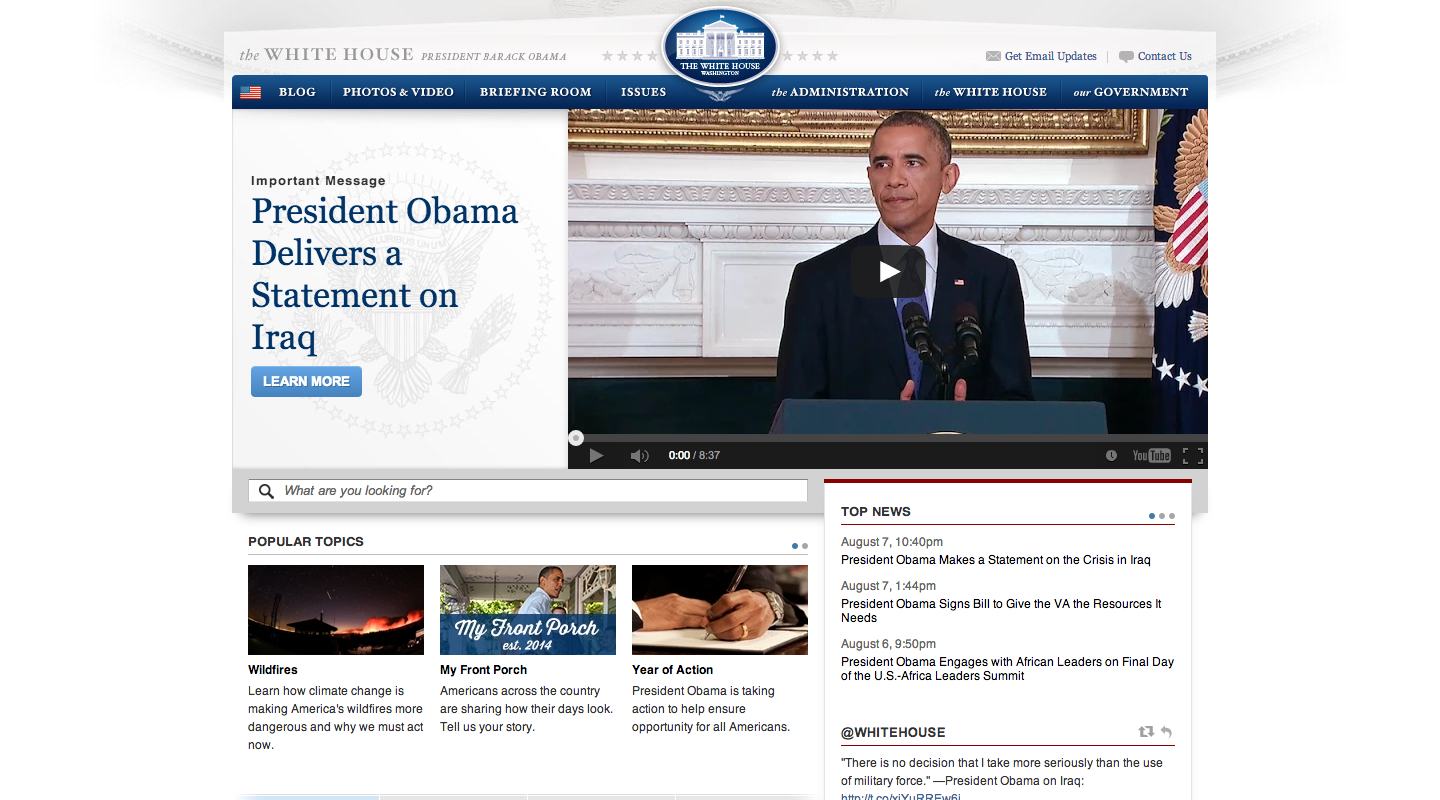
\includegraphics[width=1.8\columnwidth]{homepage-visible}}
\caption[Homepage]{Homepage of \thesite{}}
\label{fig:homepage} 
\end{figure}

The first view of the homepage has a layout scanning time enough low to shows the 6w's in the limit time of 30 seconds; the 6w's\footnote{included ``How'', \url{http://en.wikipedia.org/wiki/Five_Ws}} axis are well structured:

\begin{itemize}%[noitemsep]
	\item \textit{Where:} where are we? \\ The subtitle isn't that decriptive but the words \emph{whitehouse} and \emph{President Barack Obama} together clearify where we are. The breadcrumb lack doesn't explain where we are positioned inside the website, this fact could create user disorientation;

	\item \textit{Who:} who represent the site? \\ In the top-left there is a subtitle explaining that the representer of the whitehouse is the President Barack Obama. Note that's an image and not plain text, this doesn't respect the common rules invalidating text advantages. \\
	The whitehouse logo is in the top-center and it includes a graphical text mentioning, another time, the white house. It correctly links to the homepage but a negative note is about the size: the text is too small and the image size doesn't respect the \emph{target size rule}\footnote{the more important an img is, the bigger it should be.}; i believe that the whitehouse logo is enough important (also as homepage link) to deserve a slightly bigger size;

	\item \textit{Why:} why should i remain in this website? \\ This is not a commercial website so we are interested in public domain infos about the white house. There're daily updates about relevant polical facts, usually located in the central slideshow;

	\item \textit{What:} what offers the site? \\ This site offers any infos and news that a citizen could request, form the President activity to issues like economy, taxes, defense and political reports;

	\item \textit{When:} this is about temporal references contained in the site. \\ The ``top news'' section contains frequently updated short news and, as mentioned above, the central slideshow offers last facts updates, often supplied with a media (e.g. picture, video, etc. ); 

	\item \textit{How:} how we can move across the website? \\ The menu is top centered and has a good centered and wide submenus. There's also a search bar at the bottom of the central slideshow.

\end{itemize}



%----------------------------------------------------------------------------------------
%	INTERNAL PAGES
%----------------------------------------------------------------------------------------

\section{Internal pages}
Most of internal pages are structured in base of the sublevel: 2\textsuperscript{nd} and 3\textsuperscript{rd} levels have their layout that seems to remain unchanged for the most part of the sublevel.
All sublevel except the homepage has a \emph{location breadcrumb} located at the bottom of the menu: it shows your position relative to the homepage.
Every page seems to be reachable from the homepage in most 3 clicks, that's why whe menu is complete and well done. 
Internal pages are reachable from different pages than the home (\emph{deep linking}) so they have to propose again the compulsory informative axis: \emph{who}/\emph{what}/\emph{where}. The website correctly respect those requirement.
Below there're the analysis of three subpages, the first one sublevel is 1 and the second and the third are 2\textsuperscript{nd} level.

	\subsection{/briefing-room}
	

	\begin{figure}[h]
	\centering 
	\centerline{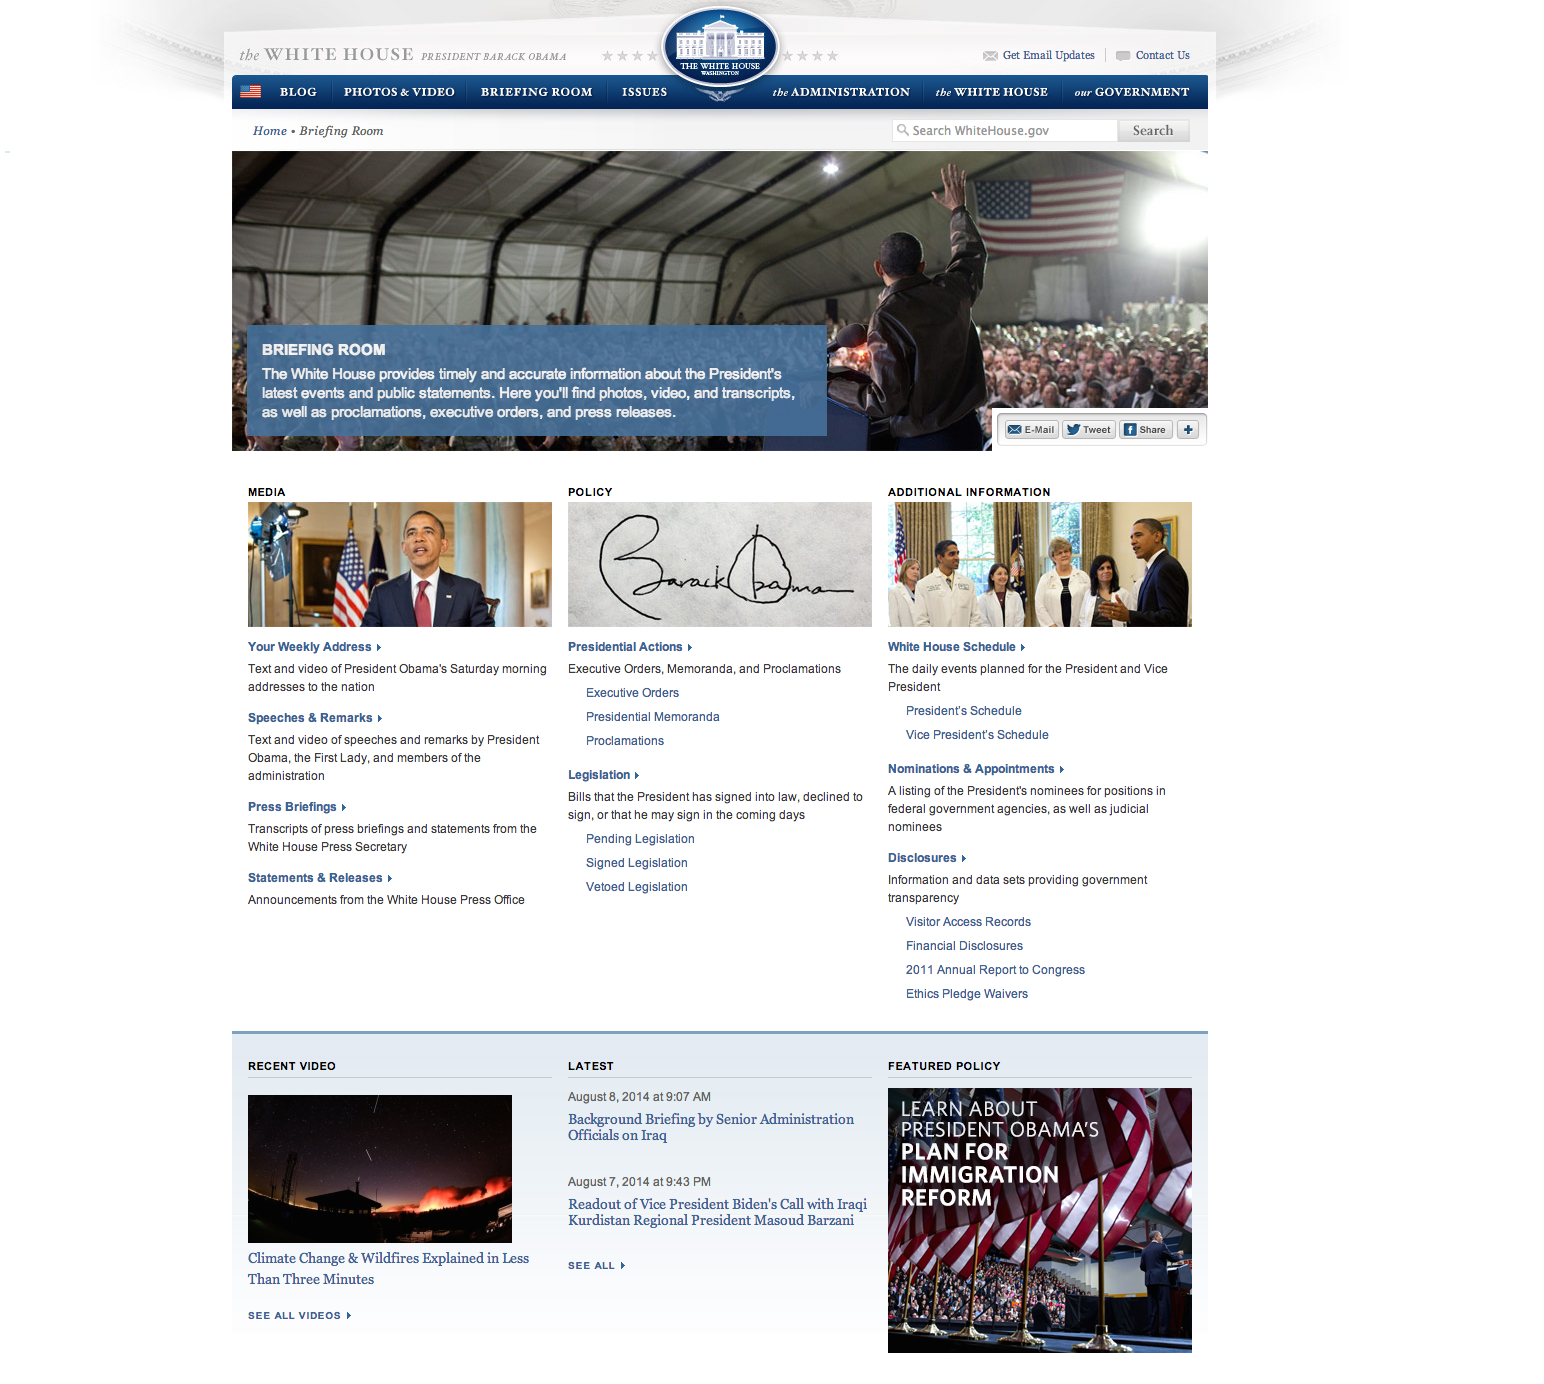
\includegraphics[width=1.8\columnwidth]{1-internal-page-entire}}
	\caption[First internal page: /briefing-room]{First internal page: \emph{/briefing-room}.}
	\label{fig:primapaginainterna} 
	\end{figure}

	The briefing room page (\href{http://www.whitehouse.gov/briefing-room}{whitehouse.gov/briefing-room}) provides informations about the President's activity, latest events and public statements. The page has a top-central wide image that immediately recall a President's public speech. A text subtitle explaining what kind of page is, that's good beacause accomplish the \emph{where} compulsory axis meanwhile permit the \emph{common text operations}\footnote{select, copy, paste.}, furthermore a set of social icons are well visible to share contents. \\
	The page content is divided in three columns, that's make user scanning effort more demanding but maybe authors wanted to put on the same footing those contents (media, policy, additional infos). Images are a bit short in height (304x125px) but sufficiently big to show their contents, they are't links so clock over doesn't produce any effects, this is undesirable since imgs appeals clicks.

	
	\subsection{/briefing-room/legislation}
	http://www.whitehouse.gov/briefing-room/legislation

	\subsection{/issues/technology}
	http://www.whitehouse.gov/issues/technology

%----------------------------------------------------------------------------------------
%	GENERALS OBSERVATIONS
%----------------------------------------------------------------------------------------

\section{General observations}


%----------------------------------------------------------------------------------------
%	SUMMARY
%----------------------------------------------------------------------------------------

\section{SUMMARY}


%----------------------------------------------------------------------------------------
%	LIST OF FIGURES
%----------------------------------------------------------------------------------------

\section{List of figures}

% %----------------------------------------------------------------------------------------
% %	
% %----------------------------------------------------------------------------------------

% \section{}



%----------------------------------------------------------------------------------------
%	BIBLIOGRAPHY
%----------------------------------------------------------------------------------------

% \renewcommand{\refname}{\spacedlowsmallcaps{References}} % For modifying the bibliography heading

% \bibliographystyle{unsrt}

% \bibliography{sample.bib} % The file containing the bibliography

%----------------------------------------------------------------------------------------

\end{document}